\documentclass[11pt,a4paper]{article}

\usepackage[a4paper,margin=0.68in,headheight=16pt]{geometry}
\usepackage[T1]{fontenc}
\usepackage{lmodern}
\usepackage[table]{xcolor}
\usepackage{graphicx}
\usepackage{tikz}
\usepackage{tabularx}
\usepackage{booktabs}
\usepackage{array}
\usepackage{enumitem}
\usepackage{float}
\usepackage{fancyhdr}
\usepackage{titlesec}
\usepackage{hyperref}
\usepackage{lastpage}
\usetikzlibrary{arrows.meta,positioning,fit,calc,backgrounds}

\definecolor{navy}{HTML}{15325B}
\definecolor{accent}{HTML}{5B5CE2}
\definecolor{accentTwo}{HTML}{0F766E}
\definecolor{lightbg}{HTML}{F5F7FB}
\definecolor{line}{HTML}{D8E2EE}
\definecolor{textgray}{HTML}{475569}
\definecolor{softpurple}{HTML}{F0ECFF}
\definecolor{softblue}{HTML}{EAF4FF}
\definecolor{softgreen}{HTML}{EAF8F3}

\hypersetup{
  colorlinks=true,
  linkcolor=navy,
  urlcolor=accent,
  pdftitle={IntellMeet AI-Powered Enterprise Meeting and Collaboration Platform},
  pdfauthor={Tanishk Mittal}
}

\pagestyle{fancy}
\fancyhf{}
\lhead{\textcolor{navy}{IntellMeet Project Report}}
\rhead{\textcolor{textgray}{Zidio Development Internship}}
\cfoot{\textcolor{textgray}{Page \thepage\ of \pageref{LastPage}}}
\renewcommand{\headrulewidth}{0.4pt}
\renewcommand{\headrule}{\hbox to\headwidth{\color{line}\leaders\hrule height \headrulewidth\hfill}}

\titleformat{\section}{\Large\bfseries\color{navy}}{\thesection}{0.6em}{}
\titleformat{\subsection}{\large\bfseries\color{navy}}{\thesubsection}{0.5em}{}
\titleformat{\subsubsection}{\normalsize\bfseries\color{accent}}{\thesubsubsection}{0.5em}{}
\titlespacing*{\section}{0pt}{0.7em}{0.35em}
\titlespacing*{\subsection}{0pt}{0.55em}{0.25em}
\setlist[itemize]{leftmargin=1.25em,itemsep=2pt,topsep=3pt}
\setlist[enumerate]{leftmargin=1.4em,itemsep=2pt,topsep=3pt}
\renewcommand{\arraystretch}{1.22}
\setlength{\parskip}{4pt}
\setlength{\parindent}{0pt}
\raggedbottom

\newcolumntype{Y}{>{\raggedright\arraybackslash}X}
\newcolumntype{L}[1]{>{\raggedright\arraybackslash}p{#1}}

\newcommand{\pill}[2]{%
  \begingroup
  \setlength{\fboxsep}{3pt}%
  \colorbox{#1}{\textcolor{navy}{\scriptsize\bfseries #2}}%
  \endgroup
}

\newcommand{\screenshotfigure}[3]{%
  \begin{figure}[H]
    \centering
    \IfFileExists{#1}{%
      \includegraphics[width=0.88\linewidth]{#1}%
    }{%
      \fcolorbox{line}{lightbg}{%
        \begin{minipage}[c][0.16\textheight][c]{0.86\linewidth}
          \centering
          \textcolor{textgray}{\textbf{Screenshot placeholder}}\\[4pt]
          \textcolor{textgray}{Add image file: \path{#1}}\\[2pt]
          \textcolor{textgray}{Keep aspect ratio and blur private data before export.}
        \end{minipage}
      }%
    }
    \caption{#2}
    \label{#3}
  \end{figure}
}

\begin{document}

% ---------------------------------------------------------------------------
% PAGE 1
% ---------------------------------------------------------------------------
\begin{titlepage}
\thispagestyle{empty}
\begin{tikzpicture}[remember picture,overlay]
  \shade[left color=navy,right color=accent] (current page.north west) rectangle ([yshift=-5.2cm]current page.north east);
  \fill[lightbg] ([yshift=-5.2cm]current page.north west) rectangle (current page.south east);
  \fill[white,opacity=0.14] ([xshift=-1.2cm,yshift=-1.2cm]current page.north east) circle (2.7cm);
  \fill[white,opacity=0.10] ([xshift=1.3cm,yshift=-4.5cm]current page.north west) circle (3.1cm);
\end{tikzpicture}

\vspace*{1.2cm}
{\color{white}\Huge\bfseries IntellMeet}\\[0.25cm]
{\color{white}\Large AI-Powered Enterprise Meeting and Collaboration Platform}\\[0.2cm]
{\color{white}\large Transforming online meetings into organized, collaborative, and actionable workspaces.}

\vfill
\begin{center}
\fcolorbox{line}{white}{%
  \begin{minipage}{0.82\linewidth}
    \vspace{0.7cm}
    \centering
    {\Large\bfseries\color{navy} Project Report}\\[0.5cm]
    \begin{tabular}{rl}
      \textbf{Author:} & Tanishk Mittal\\
      \textbf{Prepared For:} & Zidio Development -- Web Development Internship\\
      \textbf{Domain:} & Full-Stack MERN Web Development\\
      \textbf{Report Date:} & July 2026\\
      \textbf{Project Type:} & Production-oriented MERN full-stack application\\
    \end{tabular}\\[0.55cm]
    \pill{softblue}{MERN Stack}\quad
    \pill{softpurple}{WebRTC}\quad
    \pill{softblue}{Socket.io}\quad
    \pill{softgreen}{AI-Assisted Collaboration}
    \vspace{0.7cm}
  \end{minipage}
}
\end{center}
\vfill
\begin{center}
{\small\color{textgray}Suggested PDF filename: \path{IntellMeet_AI_Powered_Meeting_Platform_Tanishk_Mittal_Zidio_2026.pdf}}
\end{center}
\end{titlepage}

% ---------------------------------------------------------------------------
% PAGE 2
% ---------------------------------------------------------------------------
\tableofcontents
\vspace{0.4cm}

\section{Executive Summary and Project Overview}
\subsection{Executive Summary}
IntellMeet is a full-stack meeting and collaboration platform developed for the Zidio Development Web Development Internship. The application combines meeting scheduling, browser-based video calls, real-time chat, screen sharing, recordings, captions, post-meeting summaries, task tracking, notifications, and analytics into one MERN-based product experience.

The project addresses a common problem in remote work: meeting outcomes are often scattered across video tools, chat applications, notes, recordings, and task managers. IntellMeet brings these activities into a single workflow so that a user can schedule a meeting, invite participants, conduct the call, preserve the discussion, and convert outcomes into follow-up work.

\subsection{Problem Statement}
Remote and hybrid teams often lose important meeting outcomes because conversations, responsibilities, recordings, and follow-up tasks are spread across different tools. This creates missed action items, weak accountability, and difficulty reviewing what happened after a meeting ends.

\subsection{Proposed Solution}
IntellMeet proposes an integrated platform where the meeting lifecycle is handled in one place. Users can create meetings, invite participants, join video calls, communicate through chat, share screens, record sessions, collect captions, generate summaries, create tasks from action items, and review analytics.

\subsection{Target Users}
The platform is suitable for remote and hybrid teams, students and project groups, startups, managers, distributed software teams, and educational organizations that need a structured way to manage meetings and follow-up work.

\subsection{Major Objectives and Business Value}
The main design objectives were to reduce scattered meeting information, improve post-meeting clarity, support real-time collaboration, provide a reusable meeting history, and connect discussion outcomes to task management. These are design objectives, not experimentally measured performance or business results.

\newpage

% ---------------------------------------------------------------------------
% PAGE 3
% ---------------------------------------------------------------------------
\section{Project Scope and Key Features}
\begin{table}[H]
\centering
\small
\rowcolors{2}{lightbg}{white}
\begin{tabularx}{\linewidth}{L{1.1cm} L{3.1cm} Y L{2.8cm}}
\toprule
\textbf{ID} & \textbf{Feature} & \textbf{Description} & \textbf{Current Implementation Status}\\
\midrule
F-01 & User registration and login & Email/password signup and login screens connected to backend routes. & Implemented\\
F-02 & JWT authentication & Access tokens authorize API calls; refresh token is stored in an httpOnly cookie and rotated. & Implemented\\
F-03 & Google OAuth authentication & Google authorization-code flow exists; redirects gracefully if provider keys are missing. & Implemented, configuration required\\
F-04 & Meeting creation and scheduling & Meeting form supports title, date, time, type, description, invite emails, and timezone. & Implemented\\
F-05 & Meeting invitations & Invitee emails are parsed; existing users are added as participants; Resend sends email when configured. & Implemented with development fallback\\
F-06 & Browser-based video meetings & WebRTC full-mesh peer connections handle camera and microphone streams. & Implemented for small groups\\
F-07 & Real-time participant presence & Socket.io rooms broadcast joins, leaves, participant count, and media state. & Implemented\\
F-08 & Real-time meeting chat & Chat messages are sent through Socket.io and persisted in MongoDB. & Implemented\\
F-09 & Screen sharing & Browser Screen Capture API replaces the outgoing video track. & Implemented\\
F-10 & Meeting recording & Host can record screen/audio with MediaRecorder and upload the file. & Implemented, browser dependent\\
F-11 & Live captions & Browser Speech Recognition captures local speech and broadcasts finalized captions. & Partially implemented\\
F-12 & Post-meeting summary & Summary records are generated from transcripts through OpenAI when configured or mock fallback otherwise. & Development fallback plus optional provider\\
F-13 & Action-item extraction & Summary response includes action items with assignees and completion state. & Development fallback plus optional provider\\
F-14 & Kanban task board & User-level board with To Do, In Progress, and Done columns; drag-and-drop movement. & Implemented\\
F-15 & Notifications & Meeting-related notifications and read/unread state are stored for users. & Implemented, limited coverage\\
F-16 & Meeting history & Meetings page lists scheduled, live, and ended meetings with filtering and search. & Implemented\\
F-17 & Analytics dashboard & Charts show meeting count, live meetings, duration, weekly frequency, and productivity proxy. & Implemented from stored data\\
F-18 & CSV export & Analytics page exports metric and weekly meeting data as CSV. & Implemented\\
\bottomrule
\end{tabularx}
\caption{Key Features and Implementation Status}
\label{tab:features}
\end{table}

\subsection{Project Scope}
The current working scope includes authentication, meeting CRUD, meeting access rules, WebRTC meeting rooms, Socket.io events, screen sharing, recording upload, transcript saving, summary generation, user-level tasks, notifications, analytics, Docker backend configuration, and CI checks.

The production-level future scope includes scalable media infrastructure, TURN configuration, production speech-to-text, stronger workspace membership, role-based meeting moderation, persistent cloud recording setup, and measured load/security testing.

\newpage

% ---------------------------------------------------------------------------
% PAGE 4
% ---------------------------------------------------------------------------
\section{Technology Stack}
\begin{table}[H]
\centering
\small
\rowcolors{2}{lightbg}{white}
\begin{tabularx}{\linewidth}{L{2.5cm} L{3.0cm} Y Y}
\toprule
\textbf{Category} & \textbf{Technology} & \textbf{Role in IntellMeet} & \textbf{Reason for Selection}\\
\midrule
Frontend & React 19 & Component-based application UI. & Suitable for interactive dashboards and meeting room state.\\
Frontend & TypeScript & Static typing for frontend code and shared response shapes. & Reduces common UI and API integration errors.\\
Frontend & Vite & Development server and production bundler. & Fast local development and optimized builds.\\
Frontend & Tailwind CSS & Utility-first styling and responsive layouts. & Enables consistent enterprise-style UI quickly.\\
Frontend state & TanStack Query & Server-state fetching, caching, and invalidation. & Helps keep meeting, summary, task, and analytics data fresh.\\
Frontend state & Zustand & Auth and theme client state. & Lightweight store for global UI state.\\
Frontend routing & React Router & Protected routing and lazy route loading. & Supports app shell navigation and direct meeting URLs.\\
Visualization & Recharts & Dashboard and analytics charts. & Simple charting integration with React.\\
Backend & Node.js + Express.js & REST API, middleware, controllers, and HTTP server. & Mature JavaScript backend stack for MERN applications.\\
Backend language & JavaScript ES modules & Actual server implementation language in the supplied code. & Matches current repository; backend TypeScript is not present.\\
Database & MongoDB & Document database for users, meetings, messages, summaries, tasks, and notifications. & Flexible schema fits meeting collaboration data.\\
ODM & Mongoose & Schema definitions, model methods, and indexes. & Provides structure on top of MongoDB.\\
Realtime & Socket.io & Signalling, presence, chat, captions, and board update events. & Reliable event transport and room abstraction.\\
Media & WebRTC & Peer-to-peer audio/video media transport. & Allows browser-to-browser media without routing video through Express.\\
Security & JWT + bcrypt & Token-based auth and password hashing. & Standard approach for protected APIs.\\
Authentication & Google OAuth & Optional social login. & Reduces friction when OAuth credentials are configured.\\
Storage & Cloudinary/local uploads & Recording artifact storage. & Cloudinary supports persistent media; local fallback helps development.\\
Testing & Vitest + Supertest & Backend API integration tests. & Works well with Express and MongoMemoryServer.\\
DevOps & GitHub Actions + Docker & CI checks and containerized backend runtime. & Supports repeatable verification and deployment preparation.\\
\bottomrule
\end{tabularx}
\caption{Technology Stack}
\label{tab:stack}
\end{table}

WebRTC and Socket.io are used for different responsibilities. WebRTC transports peer-to-peer audio, video, and shared-screen media between browsers. Socket.io handles signalling messages, meeting events, participant presence, chat, captions, and board notifications.

\newpage

% ---------------------------------------------------------------------------
% PAGE 5
% ---------------------------------------------------------------------------
\section{System Architecture}
IntellMeet follows a layered MERN architecture. The browser runs the React and TypeScript frontend, which communicates with the backend through REST APIs and Socket.io. Express handles authentication, protected routes, business logic, and upload handling. MongoDB stores application data, while external services support OAuth, email, AI summaries, and media storage when configured.

\begin{figure}[H]
\centering
\resizebox{\linewidth}{!}{%
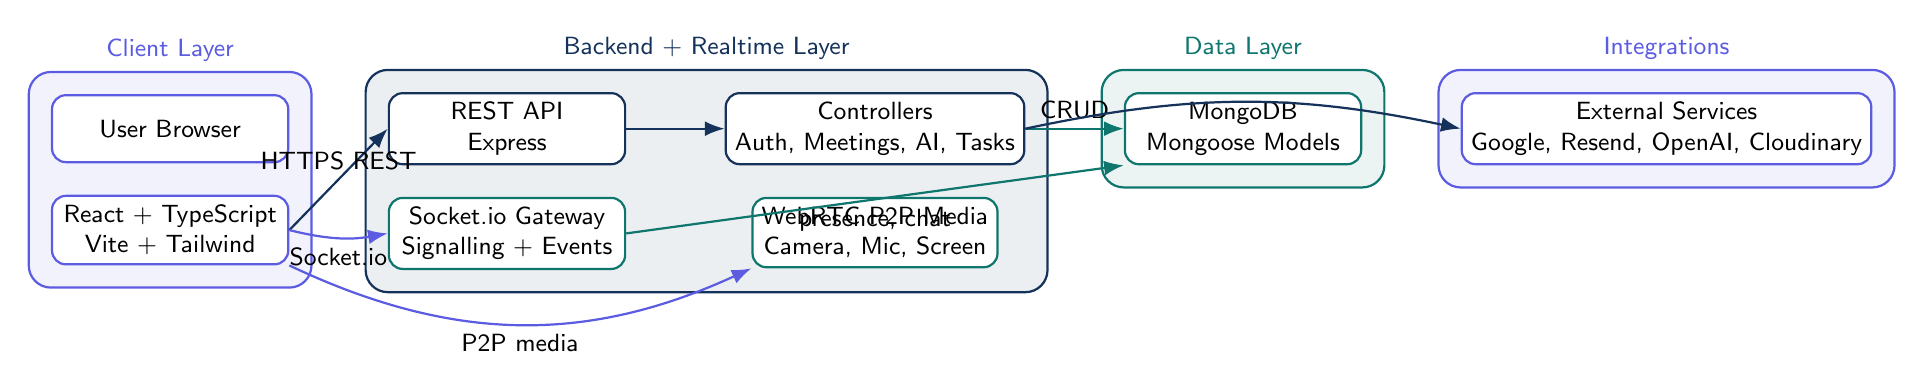
\begin{tikzpicture}[
  font=\sffamily\small,
  box/.style={rounded corners=5pt,draw=#1,fill=white,thick,align=center,minimum width=3.0cm,minimum height=0.85cm},
  group/.style={rounded corners=8pt,draw=#1,fill=#1!8,thick,inner sep=8pt},
  flow/.style={-{Latex[length=2.5mm]},thick,draw=navy},
  rflow/.style={-{Latex[length=2.5mm]},thick,draw=accent},
  dflow/.style={-{Latex[length=2.5mm]},thick,draw=accentTwo}
]
\node[box=accent] (browser) {User Browser};
\node[box=accent,below=0.4cm of browser] (react) {React + TypeScript\\Vite + Tailwind};
\node[box=navy,right=1.25cm of browser] (rest) {REST API\\Express};
\node[box=accentTwo,below=0.4cm of rest] (socket) {Socket.io Gateway\\Signalling + Events};
\node[box=navy,right=1.25cm of rest] (controllers) {Controllers\\Auth, Meetings, AI, Tasks};
\node[box=accentTwo,below=0.4cm of controllers] (webrtc) {WebRTC P2P Media\\Camera, Mic, Screen};
\node[box=accentTwo,right=1.25cm of controllers] (mongo) {MongoDB\\Mongoose Models};
\node[box=accent,right=1.25cm of mongo] (external) {External Services\\Google, Resend, OpenAI, Cloudinary};
\begin{scope}[on background layer]
  \node[group=accent,fit=(browser)(react),label={[text=accent]above:Client Layer}] {};
  \node[group=navy,fit=(rest)(socket)(controllers)(webrtc),label={[text=navy]above:Backend + Realtime Layer}] {};
  \node[group=accentTwo,fit=(mongo),label={[text=accentTwo]above:Data Layer}] {};
  \node[group=accent,fit=(external),label={[text=accent]above:Integrations}] {};
\end{scope}
\draw[flow] (react.east) -- node[above]{HTTPS REST} (rest.west);
\draw[rflow] (react.east) to[bend right=12] node[below]{Socket.io} (socket.west);
\draw[rflow] (react.south east) to[bend right=25] node[below]{P2P media} (webrtc.south west);
\draw[flow] (rest.east) -- (controllers.west);
\draw[dflow] (controllers.east) -- node[above]{CRUD} (mongo.west);
\draw[dflow] (socket.east) -- node[below]{presence, chat} (mongo.south west);
\draw[flow] (controllers.east) to[bend left=12] (external.west);
\end{tikzpicture}}
\caption{High-Level Architecture of the IntellMeet Platform}
\label{fig:architecture}
\end{figure}

\subsection{Architecture Components}
\textbf{Client Layer:} The React frontend contains authentication pages, dashboard, meetings, meeting room, recordings, AI intelligence, board, notifications, analytics, and theme controls. TanStack Query manages server state and Zustand stores auth/theme state.

\textbf{REST API Layer:} Express routes are organized into auth, meetings, AI, tasks, and misc modules. Controllers perform validation, authorization checks, persistence, and response shaping.

\textbf{Real-Time Communication Layer:} Socket.io authenticates sockets with JWTs and manages meeting rooms. It relays WebRTC offers, answers, ICE candidates, presence, chat, captions, media state, and board update events.

\textbf{Authentication Layer:} Local authentication uses bcrypt password hashing, JWT access tokens, and a hashed refresh token stored in an httpOnly cookie. Google OAuth exists as an optional configured provider.

\textbf{Data Layer:} MongoDB stores users, meetings, messages, summaries, tasks, and notifications through Mongoose models.

\textbf{Media and Recording Layer:} WebRTC media flows peer-to-peer between browsers. Meeting recordings are uploaded to Cloudinary when credentials are configured, otherwise they are written to local server uploads for development.

\textbf{AI and Speech Processing Layer:} Live captions use browser Speech Recognition. Summaries use OpenAI when an API key is configured, otherwise the backend returns a mock/template-based response with the same data shape.

\textbf{Deployment Layer:} The repository includes backend Docker configuration, docker-compose for MongoDB plus server, GitHub Actions CI, and placeholders for frontend/backend hosting URLs.

Figure~\ref{fig:auth} should be replaced with the final authentication screenshot after export from the running application. Additional recommended interface files are \path{docs/screenshots/02-dashboard.png} and \path{docs/screenshots/03-schedule-meeting.png}.

\screenshotfigure{docs/screenshots/01-authentication.png}{IntellMeet authentication interface with email/password and Google OAuth entry points.}{fig:auth}

\newpage

% ---------------------------------------------------------------------------
% PAGE 6
% ---------------------------------------------------------------------------
\section{Database and Backend Design}
The backend follows a route-controller-model structure. Routes define URL boundaries, controllers implement application logic, middleware handles authentication and errors, and Mongoose models define persistent data. The server also configures Helmet, CORS, cookie parsing, JSON parsing, static upload serving, logging, and global API rate limiting.

\begin{table}[H]
\centering
\small
\rowcolors{2}{lightbg}{white}
\begin{tabularx}{\linewidth}{L{2.4cm} Y Y}
\toprule
\textbf{Model} & \textbf{Purpose} & \textbf{Important Fields}\\
\midrule
User & Stores local and Google-authenticated users. & name, email, password hash, authProvider, googleId, avatar, role, refreshTokenHash\\
Meeting & Stores scheduled, live, and ended meetings. & code, title, date, time, scheduledAt, timezone, type, description, emails, host, participants, status, startedAt, endedAt, recordingUrl, attendees\\
Message & Stores meeting chat history. & meeting, sender, senderName, text, timestamps\\
Summary & Stores transcript, generated summary, key points, and action items. & meeting, transcript, summary, keyPoints, actionItems, accuracy, generatedBy\\
Task & Stores user-level Kanban board tasks. & owner, title, description, status, priority, assignee, order, fromMeeting\\
Notification & Stores user notifications. & user, title, message, type, read, timestamps\\
\bottomrule
\end{tabularx}
\caption{Database Models}
\label{tab:models}
\end{table}

There is no separate \texttt{Recording} model in the current source code. A recording is represented by \texttt{Meeting.recordingUrl}; related transcript and summary information is stored in the \texttt{Summary} model.

\subsection{Backend Modules}
The REST API is mounted under \texttt{/api}. Authentication routes handle signup, login, refresh, logout, current-user lookup, forgot-password stub, and Google OAuth redirects. Meeting routes handle listing, creation, updates, deletion, start/end status, recording upload, transcript saving, message history, and recording artifact listing. AI routes handle summary generation, fetching summaries, toggling action items, and a simple assistant chat endpoint. Task and misc routes handle the board, notifications, analytics, and profile updates.

\subsection{Authentication Workflow}
\begin{enumerate}
  \item The user submits credentials from the frontend.
  \item The backend finds the user and validates the password with bcrypt.
  \item Access and refresh tokens are generated.
  \item The access token authorizes protected API requests through the \texttt{Authorization} header.
  \item The refresh token is stored as an httpOnly cookie; its hash is stored on the user document.
  \item When the access token expires, the client attempts \texttt{/api/auth/refresh} and replays the failed request.
\end{enumerate}

Meeting access is checked by host, participant membership, and invited email matching. Socket.io joins also verify membership and meeting availability. The meeting model includes a 15-minute join window before start time and a 15-minute grace window after ending.

\newpage

% ---------------------------------------------------------------------------
% PAGE 7
% ---------------------------------------------------------------------------
\section{Real-Time Meeting Implementation}
Meeting creation begins in the scheduling form, which sends title, date, time, type, description, invited emails, timezone, and scheduled timestamp to the backend. The backend creates a human-readable meeting code such as \texttt{MT-xxxxx}, adds the host as a participant, resolves invited users when they already exist, creates notifications, and sends invite emails when the email provider is configured.

When a user joins a meeting room, the frontend checks whether the meeting is joinable. The room opens 15 minutes before the scheduled start time, remains available while live, and remains joinable for a short grace period after ending. The frontend requests camera and microphone access using MediaDevices. If access is denied, the user can still connect in a receive-only style session.

WebRTC manages peer-to-peer media. Socket.io does not carry video streams; it relays offers, answers, and ICE candidates so browsers can establish direct media connections. The current implementation is a full-mesh design and is appropriate for small-group demonstrations. A larger production meeting system would require an SFU such as LiveKit, mediasoup, or Janus, plus TURN configuration for restrictive networks. Figure~\ref{fig:meetingroom} documents the live meeting controls, while Figure~\ref{fig:chatcaptions} should show the collaboration panel or captions/recording area.

\screenshotfigure{docs/screenshots/04-meeting-room.png}{Live WebRTC meeting interface with camera, microphone, screen sharing, captions, chat, and recording controls.}{fig:meetingroom}

\screenshotfigure{docs/screenshots/05-chat-captions-recording.png}{Socket.io-based meeting collaboration features including chat, captions, participant state, or recording controls.}{fig:chatcaptions}

\subsection{Meeting Room Features}
The meeting room supports camera and microphone controls, screen sharing through the Screen Capture API, remote peer rendering, participant count, media state updates, host-only start/end actions, host-only recording upload, real-time chat, and browser Speech Recognition captions. Recording uses \texttt{MediaRecorder} on a display stream. When recording stops, the file is uploaded to \texttt{/api/meetings/:code/recording}. Captions collected during the meeting can be saved as transcript text before the host ends the meeting.

\newpage

% ---------------------------------------------------------------------------
% PAGE 8
% ---------------------------------------------------------------------------
\section{AI-Assisted Meeting Intelligence}
The post-meeting intelligence workflow starts from captions or transcript text. Transcript data can be saved to the backend, used to generate a summary, and displayed later in the meeting details, recordings page, or AI Intelligence page. Action items can be checked off or converted into Kanban board tasks.

\begin{enumerate}
  \item Captions or transcript data are collected in the meeting room.
  \item Transcript information is saved under the related meeting summary record.
  \item A concise summary is generated.
  \item Action items are identified with assignee text.
  \item Meeting outcomes are displayed on the AI Intelligence page and meeting details.
  \item Action items may be transferred to the task board.
\end{enumerate}

\screenshotfigure{docs/screenshots/06-ai-summary-action-items.png}{AI-assisted post-meeting summary and extracted action items.}{fig:ai}

\begin{table}[H]
\centering
\small
\rowcolors{2}{lightbg}{white}
\begin{tabularx}{\linewidth}{L{3.0cm} Y Y}
\toprule
\textbf{Capability} & \textbf{Current Method} & \textbf{Production Improvement}\\
\midrule
Transcription & Browser Speech Recognition captures finalized local speech lines and broadcasts captions. & Add a production speech-to-text service with diarization and browser-independent support.\\
Summary generation & OpenAI Chat Completions path exists when \texttt{OPENAI\_API\_KEY} is configured; otherwise mock summary fallback is used. & Add prompt validation, retry strategy, monitoring, and consistent schema validation.\\
Action-item extraction & Same summary response includes action items with assignee strings and done state. & Improve extraction with richer meeting context, due dates, and user mapping.\\
Speaker identification & Caption lines include participant display names from the local browser and socket user. & Add reliable speaker diarization from audio streams.\\
Accuracy evaluation & The displayed accuracy value is generated by the summary response and is not an experimentally measured metric. & Add a real evaluation process with labeled transcripts and quality scoring.\\
\bottomrule
\end{tabularx}
\caption{AI Capability and Production Improvement}
\label{tab:ai}
\end{table}

The current AI implementation should be described as optional provider integration with a development fallback. If no production AI key is configured, the system still demonstrates the UI and data flow using mock/template-based output. Figure~\ref{fig:ai} should show the summary, key points, and action items together.

\newpage

% ---------------------------------------------------------------------------
% PAGE 9
% ---------------------------------------------------------------------------
\section{Collaboration, Tasks, and Analytics}
The collaboration workflow continues after a meeting ends. Users can review recordings, transcripts, summaries, and extracted action items. The Kanban board stores tasks owned by the current user and supports creation, deletion, priority labels, assignee text, column movement, and optional linking back to a meeting code. Figure~\ref{fig:kanban} should show the task board columns.

\screenshotfigure{docs/screenshots/07-kanban-board.png}{Task management board for tracking meeting outcomes.}{fig:kanban}

The board is currently user-level rather than a full organization workspace with membership roles. Socket.io includes a workspace-style event for task changes, but the current workspace identifier is the user ID. Therefore, it should be presented as a personal or user-level board in the report.

\screenshotfigure{docs/screenshots/08-analytics-history.png}{Meeting engagement analytics and historical meeting data.}{fig:analytics}

Analytics are derived from stored meeting and summary data. The backend computes total meetings, live meetings, average ended-meeting duration, weekly meeting frequency, and a productivity score based on action-item completion when available. The frontend visualizes this data using Recharts and includes a CSV export for analytics metrics and weekly counts. Figure~\ref{fig:analytics} should show analytics, meeting history, or recording history.

Notifications are stored per user and can be marked read individually or in bulk. Meeting history is searchable and filterable by status. The recordings page lists recordings from meetings the user hosted or was invited to, and supports opening the recording, copying its link, downloading the transcript, or jumping to the summary page.

\newpage

% ---------------------------------------------------------------------------
% PAGE 10
% ---------------------------------------------------------------------------
\section{Security, Privacy, and Performance}
\subsection{Authentication Security}
Passwords are hashed with bcrypt before storage. The access token is kept in frontend memory rather than localStorage. The refresh token is stored in an httpOnly cookie and its hash is stored in the database. Refresh tokens are rotated during refresh and cleared during logout.

\subsection{Authorization}
Protected REST routes use JWT middleware. Meeting operations check whether the user is the host, participant, or invited email member depending on the action. Start, end, update, delete, recording upload, and transcript save operations are host-restricted where appropriate.

\subsection{API Security}
The Express app uses Helmet, CORS configured through \texttt{CLIENT\_ORIGIN}, cookie parsing, JSON body limits, centralized error handling, global API rate limiting, and stricter auth route rate limiting. File uploads are restricted to \texttt{webm}, \texttt{mp4}, or browser-compatible audio/video MIME types with a 100 MB limit.

\subsection{Data Protection and Environment Variables}
Secrets are read from environment variables. The repository includes a safe \texttt{.env.example} with placeholder values. The report must not include real secrets, API keys, tokens, meeting links, or private email addresses in screenshots.

\subsection{Frontend Security}
Protected routes require authenticated user state. Axios interceptors attach access tokens and perform silent refresh on 401 responses. Google OAuth returns the access token through the URL fragment, which avoids query-string logging.

\subsection{Performance Optimizations}
The frontend uses Vite production builds, route-level lazy loading, server-state caching with TanStack Query, and chart components loaded at route level. The backend uses MongoDB indexes on important fields such as email, meeting code, owner, status, and meeting references. Build output is compressed by modern hosting platforms, but measured deployment performance is still pending.

\subsection{Accessibility and Responsive Design}
The UI uses semantic buttons, form labels, icon button labels, responsive grids, and mobile-friendly layouts. Further accessibility verification should be completed with keyboard testing and Lighthouse.

\begin{table}[H]
\centering
\small
\rowcolors{2}{lightbg}{white}
\begin{tabularx}{\linewidth}{L{4.2cm} Y}
\toprule
\textbf{Metric} & \textbf{Value}\\
\midrule
Lighthouse Performance & [Add score]\\
Lighthouse Accessibility & [Add score]\\
Initial Page Load & [Add measured value]\\
Backend API Response Time & [Add measured value]\\
\bottomrule
\end{tabularx}
\caption{Performance and Accessibility Measurement Placeholders}
\label{tab:metrics}
\end{table}

\newpage

% ---------------------------------------------------------------------------
% PAGE 11
% ---------------------------------------------------------------------------
\section{Testing, Deployment, and DevOps}
The project includes frontend and backend verification steps. The frontend supports TypeScript checking, ESLint, formatting, and production builds. The backend uses Vitest, Supertest, and MongoMemoryServer to test API behavior with an isolated in-memory database. A GitHub Actions workflow runs frontend lint, typecheck, build, and backend tests on pushes and pull requests to \texttt{main}.

\begin{table}[H]
\centering
\small
\rowcolors{2}{lightbg}{white}
\begin{tabularx}{\linewidth}{L{3.0cm} L{3.2cm} Y L{3.0cm}}
\toprule
\textbf{Test Type} & \textbf{Tool/Method} & \textbf{Area Tested} & \textbf{Result}\\
\midrule
Frontend type validation & \texttt{npm run typecheck} & TypeScript frontend compilation. & Passed locally\\
Frontend lint & \texttt{npm run lint} & React/TypeScript lint rules. & Passed with 2 warnings\\
Frontend production build & \texttt{npm run build} & TypeScript project build and Vite bundle generation. & Passed locally\\
Backend API tests & Vitest + Supertest + MongoMemoryServer & Health, auth, meetings, recordings, transcripts, timing rules, tasks, and AI fallback. & Passed locally: 14 tests\\
Manual multi-user meeting test & Browser sessions & WebRTC, Socket.io, screen share, captions, recording. & Partially verified; requires final demo pass\\
Deployment smoke test & Hosted URLs & Frontend, backend, database, OAuth, uploads. & Requires deployment testing\\
\bottomrule
\end{tabularx}
\caption{Testing Summary}
\label{tab:testing}
\end{table}

\subsection{Deployment Preparation}
The backend includes a Dockerfile with a non-root runtime user and a container health check against \texttt{/api/health}. The docker-compose file can run MongoDB and the backend together for local/container testing. Production deployment can use Vercel or another frontend platform, Render/Railway or another backend platform, and MongoDB Atlas.

\begin{table}[H]
\centering
\small
\begin{tabularx}{\linewidth}{L{4.0cm} Y}
\toprule
\textbf{Deployment Item} & \textbf{Value}\\
\midrule
Frontend URL & [Add deployed frontend URL]\\
Backend API URL & [Add backend API URL]\\
GitHub Repository & [Add GitHub repository URL]\\
Demo Video & [Add demo video URL]\\
\bottomrule
\end{tabularx}
\caption{Deployment Links to Complete Before Submission}
\label{tab:deployment}
\end{table}

Figure~\ref{fig:deployment} should be replaced by either the deployed application screen or the GitHub Actions CI result before submission.

\screenshotfigure{docs/screenshots/09-deployment-ci.png}{Deployed application screen or CI/CD pipeline result.}{fig:deployment}

\newpage

% ---------------------------------------------------------------------------
% PAGE 12
% ---------------------------------------------------------------------------
\section{Challenges, Limitations, Future Roadmap, and Reflection}
\subsection{A. Challenges Faced}
\textbf{WebRTC connection setup:} The main challenge was coordinating browser media streams with Socket.io signalling. The cause was that peer connections require a strict offer, answer, and ICE candidate flow. The solution was to split initiator responsibility: existing participants receive offers from newcomers, while newcomers initiate offers to existing peers. I learned that signalling and media transport must be designed separately.

\textbf{Participant state synchronization:} Presence, mute/camera state, joins, leaves, and disconnect cleanup had to stay consistent across clients. Socket.io rooms and server-side maps were used to broadcast participant updates. I learned the importance of cleaning up socket state when users leave or refresh.

\textbf{Recording browser streams:} Recording depends on browser permission, supported codecs, and the user choosing a screen/window. The workaround was to use \texttt{MediaRecorder} with supported MIME type detection and upload the resulting blob. I learned that browser media APIs behave differently across environments.

\textbf{Token refresh handling:} The frontend needed to recover from expired access tokens without forcing frequent logins. Axios interceptors were used to refresh once and replay failed requests. I learned to separate short-lived access tokens from long-lived refresh cookies.

\textbf{AI fallback management:} The system needed to work without paid API keys. The backend therefore supports a mock summary fallback while keeping the same response shape as the optional OpenAI path. I learned to document fallback behavior honestly.

\subsection{B. Current Limitations}
\begin{table}[H]
\centering
\small
\rowcolors{2}{lightbg}{white}
\begin{tabularx}{\linewidth}{Y Y}
\toprule
\textbf{Current Limitation} & \textbf{Future Improvement}\\
\midrule
Peer-to-peer mesh does not scale well to large meetings. & Add an SFU such as LiveKit, mediasoup, or Janus.\\
TURN server is not configured in the current client. & Configure TURN for restrictive NAT and corporate networks.\\
Live captions depend on browser Speech Recognition support. & Add a production speech-to-text provider.\\
AI functionality may use mock fallback without \texttt{OPENAI\_API\_KEY}. & Configure production AI provider and validate responses.\\
Local recording storage may not persist on cloud hosting. & Use Cloudinary or another persistent media store in production.\\
Task board is user-level, not full team workspace membership. & Add organizations, teams, roles, and user assignment.\\
Forgot-password route is a non-enumerating stub. & Implement reset tokens and email delivery.\\
Measured load testing is pending. & Add load, security, and browser compatibility testing.\\
\bottomrule
\end{tabularx}
\caption{Current Limitations and Future Improvements}
\label{tab:limitations}
\end{table}

\subsection{C. Future Roadmap}
Future improvements include SFU integration, TURN server configuration, production speech-to-text, improved AI action-item extraction, real team workspaces, user-based task assignment, calendar integration, persistent cloud recording, meeting search, role-based moderation, end-to-end encryption research, a mobile application, and automated load/security testing.

\subsection{D. Personal Reflection}
While developing IntellMeet, I improved my understanding of full-stack architecture and how frontend, backend, database, and real-time systems interact. Working with WebRTC and Socket.io helped me understand the difference between media transport and signalling. I also learned how secure authentication is built using hashed passwords, JWT access tokens, refresh-token rotation, and protected routes.

The project gave me practical experience with asynchronous application state, browser media APIs, API error handling, and deployment planning. I also learned to distinguish between a working prototype and production-grade infrastructure. Features such as AI summaries, captions, and recordings are useful, but they require careful provider configuration, storage decisions, and testing before production use.

Overall, IntellMeet helped me improve my debugging, documentation, project planning, and technical decision-making skills. The project demonstrates a meaningful MERN application while also making clear which areas need further engineering before large-scale production use.

\newpage

% ---------------------------------------------------------------------------
% PAGE 13
% ---------------------------------------------------------------------------
\section{Conclusion, Checklist, and Missing Values}
\subsection{Project Conclusion}
IntellMeet successfully demonstrates an integrated meeting and collaboration workflow using a MERN-based architecture. The current application includes authentication, scheduling, real-time meeting communication, chat, screen sharing, recording upload, transcript saving, AI-assisted summary generation with fallback support, task tracking, notifications, analytics, CI checks, and backend container configuration.

The project is suitable as a submission-ready internship project because it shows practical full-stack engineering, real-time communication, database modeling, frontend state management, and honest production planning. Its limitations are clearly documented, especially around large-scale WebRTC infrastructure, speech recognition reliability, production AI configuration, and deployment verification.

\subsection{Header and Footer Suggestions}
The report source already uses a professional header and footer. The header shows \textit{IntellMeet Project Report} on the left and \textit{Zidio Development Internship} on the right. The footer shows page numbers in the format \textit{Page X of Y}. This should be retained for PDF export.

\subsection{Final Submission Checklist}
\begin{itemize}
  \item Replace all screenshot placeholders with clean, cropped screenshots.
  \item Blur personal emails, tokens, meeting links, API keys, and private information.
  \item Add deployed frontend and backend URLs after hosting.
  \item Add GitHub repository and demo video URLs.
  \item Add Lighthouse and API response measurements after deployment.
  \item Compile the report in Overleaf using pdfLaTeX.
  \item Confirm the PDF file size remains below 10 MB.
  \item Review all figure captions and table numbers before submission.
  \item Confirm no unsupported claims about Kubernetes, Redis, Grafana, Prometheus, AWS, TURN, or SFU infrastructure are present.
\end{itemize}

\subsection{Missing Values to Complete Manually}
\begin{table}[H]
\centering
\small
\rowcolors{2}{lightbg}{white}
\begin{tabularx}{\linewidth}{L{4.2cm} Y}
\toprule
\textbf{Missing Value} & \textbf{Placeholder}\\
\midrule
Frontend deployment & [Add deployed frontend URL]\\
Backend deployment & [Add backend API URL]\\
GitHub repository & [Add GitHub repository URL]\\
Demo video & [Add demo video URL]\\
Lighthouse Performance & [Add score]\\
Lighthouse Accessibility & [Add score]\\
Initial Page Load & [Add measured value]\\
Backend API Response Time & [Add measured value]\\
Screenshots & Add files under \path{docs/screenshots/} using the filenames shown in figure placeholders.\\
\bottomrule
\end{tabularx}
\caption{Manual Completion List}
\label{tab:missing}
\end{table}

\subsection{Consistency Check}
\begin{itemize}
  \item Technologies match the inspected source code: React, TypeScript frontend, Vite, Tailwind CSS, Zustand, TanStack Query, Express JavaScript backend, MongoDB, Mongoose, Socket.io, WebRTC, Vitest, Docker, and GitHub Actions.
  \item Features match implemented routes, pages, models, and hooks.
  \item No secret values are included.
  \item Unimplemented or provider-dependent features are marked as fallback, partial, planned, or configuration required.
  \item Figure numbers are sequential and every figure has a caption.
  \item Screenshot placeholders are included because no screenshot image files were available in the uploaded attachments.
  \item The report is designed for 13 A4 portrait pages, keeping within the requested 10--13 page range.
  \item PDF size should remain below 10 MB if screenshots are compressed before insertion.
\end{itemize}

\end{document}
